\chapter{Backprop In Practice}\label{chp:Backprop in Practice}
% Authors: tn1050@nyu.edu, vy404@nyu.edu, sk7685@nyu.edu.
% Lecture date: 2.4.19
\setlength{\abovedisplayskip}{7pt}
\setlength{\belowdisplayskip}{7pt}

% Authors: tn1050@nyu.edu, vy404@nyu.edu, sk7685@nyu.edu.
% Lecture date: 2.4.19
\section{Use of ReLU non-linearities}
Non-linear transformations are an essential part of the deep neural networks as discussed in the Chapter 3. An artificial neuron does not know the bounds of its values and can not decide whether it should fire or not, we use activation functions to check the value 
\begin{equation}
    Y = \sum (W * X_{in}) + C
\end{equation}

produced by the neuron and decide if the neuron is fired or not. 
\begin{enumerate}[label=(\alph*)]
\item The step function is a threshold based activation function Activation function. 
\begin{equation}
    f(x)=\begin{cases}
            activated, & Y > threshold
            deactivated, & Y < threshold
        \end{cases}
\end{equation}

However the step function does not account for partial activation which can help learning become smoother and easier (less wiggly). It also has zero gradients, which makes it hard to train in practical setting. As an alternative, people used sigmoid or hyperbolic tangent non-linearities in neural networks, which are saturating functions. 
\begin{figure}[ht]
\centering
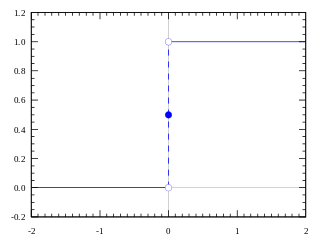
\includegraphics[width=50mm]{lectures/02-b/step_function.png}
\caption{Unit Step Function}
\label{fig:step_function}
\end{figure}

\item The sigmoid function is a mathematical function having an "S" shaped curve (sigmoid curve).
\begin{equation}
    f(x) = \frac{1}{1+e^{-x}}
\end{equation}
has a problem of vanishing gradients towards either end of the function causing the network to stop learning or to learn at a very slow rate.

\begin{figure}[ht]
\centering
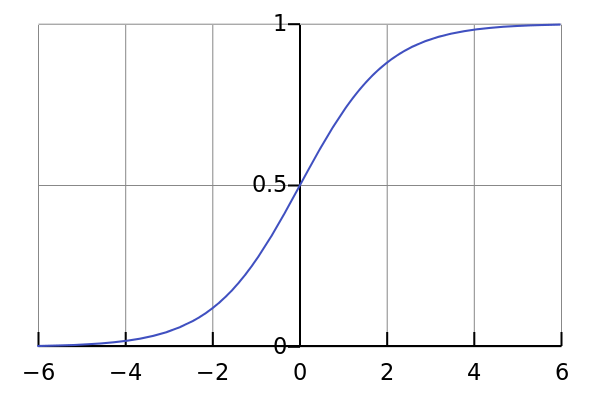
\includegraphics[width=50mm]{lectures/02-b/sigmoid_function.png}
\caption{Sigmoid Function}
\label{fig:sigmoid}
\end{figure}

\item The tanh function also has vanishing gradient characteristics similar to sigmoid function,
\begin{equation}
    f(x) = \frac{2}{(1+e^{-2x})}-1
\end{equation}
but it presents an improvement over the sigmoid by extending to negative values and avoiding bias in the gradients. 
However its gradient characteristics hinders our ability to train deeper neural network and for this reason, they fell out of favor and using ReLU non-linearities enabled us to train much deeper networks. 

\begin{figure}[ht]
\centering
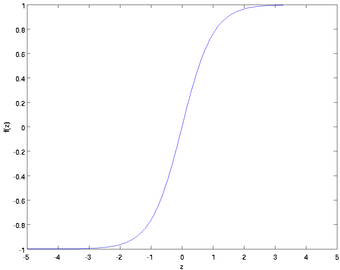
\includegraphics[width=50mm]{lectures/02-b/tanh_function.png}
\caption{tanh Function}
\label{fig:tanh}
\end{figure}

\item The Rectified Linear Unit is an activation function defined as 
\begin{equation}
    f(x) = \max (0,x)
\end{equation}
where x is the input to a neuron giving an output x if x is positive and 0 otherwise. 
This promotes a reduced likelihood of encountering vanishing gradient problems. When $a > 0$, the gradient has a constant value. 
In contrast, the gradient of sigmoids becomes increasingly small as the absolute value of x increases.
The constant gradient of ReLUs results in faster learning.

ReLU also helps with increasing the sparsity of the network which arises when $a ≤ 0$. 
As the number of such units increase in a layer, it leads to a sparse representation. 
Sigmoids on the other hand are always likely to generate some non-zero value resulting in dense representations. 
The range of values can also be infinite.

ReLU is analogous to half-wave rectification in electrical engineering and has been the most popular activation function to this day.

\begin{figure}[ht]
\centering
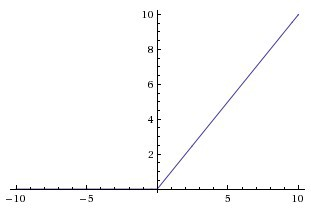
\includegraphics[width=50mm]{lectures/02-b/ReLU_function.jpg}
\caption{ReLU Function}
\label{fig:relu}
\end{figure}
\end{enumerate}

{\centering\fbox{\begin{minipage}{30em}
\centering\textbf{Use of ReLU non-linearities}
\begin{enumerate}
    \item ReLU nonlinearities learns much faster than the standard sigmoid function and improves our ability to train deeper neural networks.
    \item Also helps with increasing the sparsity of network as the neuron is switched off for $a \leq 0$
\end{enumerate}
\end{minipage}}\par}

% Authors: tn1050@nyu.edu, vy404@nyu.edu, sk7685@nyu.edu. 
% Lecture date: 2.4.19
\section{Use cross-entropy loss for classification}
When we work on classification problems we use cross-entropy loss which measures performance of a classification model whose output is a probability value. 
The cross entropy loss increases as the predicted probability moves away from the actual label. 
Log loss penalizes all errors however gives higher penalty to the predictions that are confident and wrong. 
It is defined as,
\begin{equation}
H(y, p)=-\sum_i y_i \log(p_i)
\end{equation}
we calculate a separate loss for each class label per observation and sum the result. 
Cross entropy measure is a widely used alternative of squared error.

Log softmax is a special case of cross entropy loss where only one value in the output array is $1$ and the others are $0$. 
The more general form calculates the cross-entropy between two discrete distributions which log-softmax doesn’t compute. 
Softmax is often the best option to use for classification problems. 

{\centering\fbox{\begin{minipage}{30em}
\centering\textbf{Use cross-entropy loss for classification}
\begin{enumerate}
    \item Cross entropy loss increases as the predicted probability moves away from the actual label.
    \item Log softmax is a special case of cross entropy loss.
\end{enumerate}
\end{minipage}}\par}
\vspace{5pt}


% Authors: tn1050@nyu.edu, vy404@nyu.edu, sk7685@nyu.edu. 
% Lecture date: 2.4.19 
\section{Use Stochastic Gradient on Minibatches}
The standard gradient descent algorithm updates the model parameters $θ$ in the following way: 
% θ=θ−α∇θE[J(θ)] 
\begin{equation}
    \theta = \theta - \alpha\bigtriangledown\theta E [J(\theta)]
\end{equation}
where the expectation in the above equation is approximated by evaluating the cost and gradient over the full training set. 
Stochastic Gradient Descent (SGD) simply does away with the expectation in the update and computes the gradient of the parameters using only a single or a few training examples. 
An estimate of the true gradient is computed based on the error $E^t$ of that example, and the weights are updated in the following way: 
% W(t+1) = W(t) - ndel E^t/del W. 
\begin{equation}
    W(t+1) = W(t) - \eta \dfrac{\delta E^t}{\delta W}
\end{equation}
Generally each parameter update in SGD is computed w.r.t a few training examples or a minibatch as opposed to a single example. 

\begin{figure}[ht]
\centering
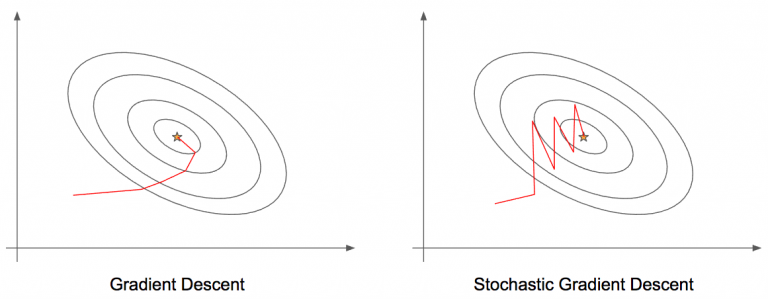
\includegraphics[width=120mm]{lectures/02-b/Stochastic.png}
\caption{Gradient Descent vs. Stochastic Gradient Descent}
\label{fig:sgd}
\end{figure}
We do forward and backward propagation on a small group of samples, compute their average gradients which are then used to update the model parameters. 
We then take the next group of samples and repeat this process. The two limit cases are when the size of the batch is one or the size of the batch is the entire training set. 
It is inefficient to use the entire training set to compute the gradient as there might be many redundant samples in the training set. 
For instance, if a training set contains one million samples which are just repetition of ten-thousand images hundred times, then by using the full batch gradient-descent we will be using hundred times the number of resources computing the gradient than we should. 

We do not have such training sets in real life. However, we often have a lot of samples that are very redundant. 
For instance, while doing character recognition on MNIST dataset, we will have a lot of ones very very similar to each other (with very minor variations). 
Similarly, ImageNet has many pictures where samples within the same category are very similar to each other. 
On large datasets, SGD can converge faster than batch training because it performs updates more frequently.
We can get away with this because the data often contains redundant information, so the gradient can be reasonably approximated without using the full dataset. 
If there were no redundancy we wouldn’t be able to learn any generalizable information.

However, in the presence of redundancy if we calculate the gradient on the entire training set we will be doing more computation than necessary. 
There has been some research done on the optimal size of a batch. 
There is an argument that small batch sizes put a lot of noise in the gradients, which in turn changes the weights more and produces a  regularization effect that leads to better generalization error.

Another factor in determining the batch size is how well we can saturate the current hardware.
Generally, the calculation in a neural net is not limited by the speed of the processor but is limited by how fast you can shuffle data in and out of the processor to and from the memory. 
Minibatch training can be faster than training on single data points because it can take advantage of vectorized operations to process the entire minibatch at once. 
How we organize the calculation within a GPU allows us to take advantage of their cache. 
One good way to optimize memory bandwidth is to use matrix multiplication at the lowest level (matrix multiplication is an operation that has a large number of operations per memory access thus we organize data in such a way that for every piece of data we load from memory we do a lot of operations with them).

In general, we use the smallest batch size that will saturate the hardware. 
Another factor that comes into consideration is parallelization. 
The simplest way to parallelize the training of a neural net is to take a large batch,  divide it into chunks and give each chunk to a separate GPU. 
Their gradients will then be averaged and used for updating the model parameters, which are then distributed to each of the workers (synchronous distributed SGD).

{\centering\fbox{\begin{minipage}{30em}
\centering\textbf{Stochastic Learning with minibatches}
\begin{enumerate}
    \item Stochastic learning is usually much faster and uses lesser resources than batch learning.
    \item Stochastic learning often results in better solutions than batch learning that produce less generalization error
    \item As a rule of thumb, we can use the samllest batch size that will saturate the hardware.
\end{enumerate}
\end{minipage}}\par}

% Authors: tn1050@nyu.edu, vy404@nyu.edu, sk7685@nyu.edu.
% Lecture date: 2.4.19
\section{Shuffle training samples} 
The optimum way of using the training data is by shuffling it in a way that each minibatch would have as much diversity as possible. 
If we were to be given a training set where the first six thousand examples are all zeros, next six thousand examples are all ones, followed by twos, threes, etc. the neural network will learn extremely slowly. 
This is because the model can completely ignore all the inputs and update its biases to output a given class. 
In this example, the model might ignore all the inputs first and learn to output zero by adjusting its biases. 
Then it will do the same for ones etc. It can be seen that this process would not update the input weights very often. 
It is, therefore, best to create diverse mini batches with our shuffling procedure. 
One way of accomplishing this would be taking an equal number of samples for each class while constructing the mini-batches. 
There is some research suggesting that the optimal size of a batch is somewhat related to the number of categories for classification problems.

One other concern is that if a type of input is underrepresented in the training data, the model would not be incentivized to learn them well. 
Often we have different categories that have different frequencies in the dataset. 
For instance, if we train the facial recognition model where the training data has a racial distribution that reflects the racial distribution of the United States, it would result in some races to be underrepresented. 
This would hinder the model’s performance on these types of inputs as it will focus on learning the dominant types of inputs. 
Eventually, it will not learn the relevant properties/features to represent those underrepresented races and would not work well for such samples.

If there is an unbalanced set of classes, one strategy that people sometimes use is downsampling. 
This should be avoided and we must try to make use of all available data. 
One way of doing this would be by picking a category at random first, and then taking a sample within that category. 
One can generate a counter for each class, which would denote the number of samples that were taken from that class so far. 
This counter would be incremented for each sample taken from that category. 
Once we reach the end of a given category, we would shuffle its samples, set its counter to zero and proceed further. 
This would equalize the frequency in a simple way while still making us able to use all the available data. 
However, it will also cause the model to assign similar probabilities to all categories however rare they may be.  
To overcome this, we can do one more pass using the real distribution of the data and re-train with real frequencies which will affect the last few layers, changing their bias and adjusting to accommodate for the real percentages. 
This is similar to what softmax does. One other strategy that one can encounter is modifying the loss function to have different weights for samples from different categories. 
However this will result in using a bigger step size for smaller underrepresented classes (that have larger multipliers) which tends to break the dynamics of the stochastic gradient descent.

{\centering\fbox{\begin{minipage}{30em}
\centering\textbf{Shuffling Training Samples}
\begin{enumerate}
    \item Shuffle training samples so that the samples in a batch belong to different classes.
    \item Present input variables that produce a large error more frequently than examples that produce a small error. Then do one more pass with real frequencies after training the model with equalized frequencies to accommodate for real data distribution.
\end{enumerate}
\end{minipage}}\par}
\vspace{5pt}

% Authors: tn1050@nyu.edu, vy404@nyu.edu, sk7685@nyu.edu.
% Lecture date: 2.4.19
\section{Normalize Input Variable} 
It is important for inputs to be normalized (having mean zero and standard deviation of one) so to make sure that the optimization well behaves and converges at a fast rate.
A shift of the average input away from zero creates a bias in the updates in a particular direction, which slows down learning. 
Because of this reason it is advisable to have a zero mean over the training set. 
Having nonzero means, create large eigenvalues. This causes the cost surface to be steep in some directions and shallow in others, which in turn would slows the convergence. 

\begin{figure}[ht]
\centering
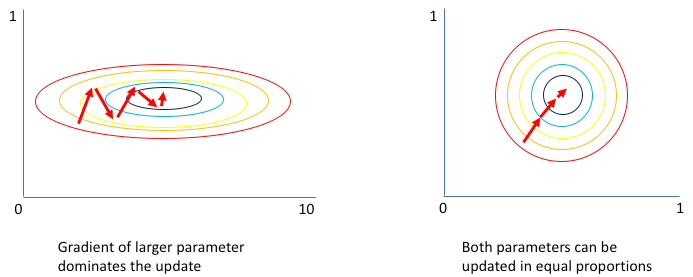
\includegraphics[width=120mm]{lectures/02-b/Why_normalize.png}
\caption{Normalizing inputs to a standard scale}
\label{fig:normalize}
\end{figure}

Another factor influencing the convergence rate is the scaling of the input variables such that they have the same covariance, as inputs that have large variations in spread along different directions of the input space do also slow down the learning. 
This speeds up learning as it helps to balance out the rate at which the weights connected to input nodes learn. 
By normalizing each layer, we are introducing a level of orthogonality between layers - which generally makes it easier for the learning process.

\begin{figure}[ht]
\centering
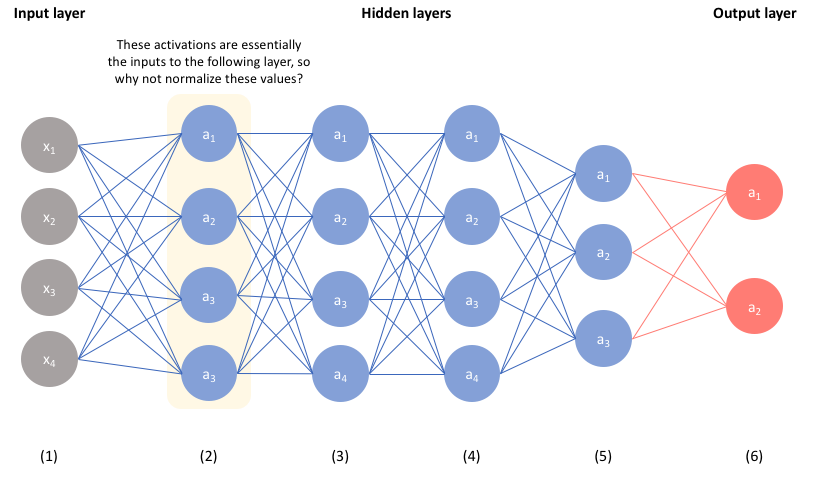
\includegraphics[width=120mm]{lectures/02-b/Benefit of normalization.png}
\caption{Normalization on each layer}
\label{fig:normalize2}
\end{figure}

There is a module called batchnorm which is used for the same and is placed before or after ReLU or both for this purpose. 
It takes the sample of the batch and normalizes input values across the minibatch. 
In addition to batchnorm, there are alternative techniques - featurenorm and goodnorm - which address this problem. 
Feature norm normalizes across the entire feature and goodnorm normalizes across the entire array.
While training neural nets with gradient-based procedures, we adjust every weight according to its gradient under the assumption that other weights remain constant. 
However, they change every iteration in practice. Changes in weights in layer $k-1$ can result in a change of inputs to layer $k$. 
After applying batch norm to the layers, we make sure that the inputs to every layer are close to the standard normal distribution easing dependencies between layers. 
To increase the stability of a neural network, batch normalization normalizes the output of a previous activation layer by subtracting the batch mean and dividing by the batch standard deviation. 
Given a vector of linear combinations from the previous layer $z[l]$ for each observation $i$ in a dataset, we can calculate the mean and variance as: 
\begin{equation}
    \mu = \frac{1}{m} \sum_i z_i^{[l]}
\end{equation}
\begin{equation}
    \sigma^2 = \frac{1}{m} \sum_i (z_i^{[l]} - \mu)^2
\end{equation}
% μ=1/m∑i z_i^[l]
% σ2=1/m∑i z_i^[l]−μ)^2
Using these values, we can normalize the vectors $z[l]$ as follows.
% z_norm^(i)=(z(i)−μ)/√(σ^2+ε)
\begin{equation}
    Z_norm^(i) = \dfrac{z(i) - \mu}{\sqrt{\sigma^2+\varepsilon}}
\end{equation}
We add a very small number ϵ to prevent the chance of a divide by zero error.

Batch norm is the most popular however is not that great as it depends on the batch size and we need to maintain a running average of mean and standard deviation which can not be done when running on test cases and we need an equivalent operation for that time. 
In goodnorm, on the other hand, we do the same operation in both testing and training. 

As a result of introducing orthogonality between layers such that we avoid shifting distributions in activations as the parameters in earlier layers are updated, we can build deeper networks using normalization.

{\centering\fbox{\begin{minipage}{30em}
\centering\textbf{Normalize Input Variables}
\begin{enumerate}
    \item The mean of each input variable over the training set should be approaching zero.
    \item Scale input variables so that their covariances are about the same.
\end{enumerate}
\end{minipage}}\par}

% Authors: tn1050@nyu.edu, vy404@nyu.edu, sk7685@nyu.edu.
% Lecture date: 2.4.19
\section{Use a bit of L1 and L2 regularization on the weights} 
The use of regularization is well studied in the machine learning literature and they are used widely in different types of learning algorithms in one form or another to avoid overfitting. 
One form of regularization we can impose on the learning algorithm would be by putting constraints on the weights, and this is usually done by adding a term to the cost function. 
To that end, we can add 
\begin{equation}
\alpha*||w||_2^2 \hspace{0.5cm}
or \hspace{0.5cm}
\beta*||w||_1 
\end{equation}
terms to the cost function to impose L2 or L1 regularizations respectively. 
This will keep the model parameters from increasing and will increase the bias to ensure the model does not have high variance (i.e., overfitting). 
It will also help to remove some of the parameters if we use L1 regularization. 
Weight regularization also help the weights to spread around. 
That has some advantages for generalization as it tends to regularize the solution so that it is more general. 
It is best to start regularization after a couple of epochs and crank it up as loss decreases so that the solution does not collapse in the beginning with all weights becoming zero.

{\centering\fbox{\begin{minipage}{30em}
\centering\textbf{Use a bit of L1 and L2 regularization on the weights}
\begin{enumerate}
    \item It keeps the model parameters from increasing and will increase the bias to ensure the model does not have high variance.
    \item Best to start regularization after a couple of epochs else all weights become zero.
\end{enumerate}
\end{minipage}}\par}

% Authors: tn1050@nyu.edu, vy404@nyu.edu, sk7685@nyu.edu.
% Lecture date: 2.4.19
\section{Use “dropout” for Regularization}
Dropout is a way of regularization that makes neural nets more robust and prevents overfitting. 
It is a layer that randomly masks out some percentage of the units in the layer and “ignores” them during a particular forward or backward pass.

\begin{figure}[ht]
\centering
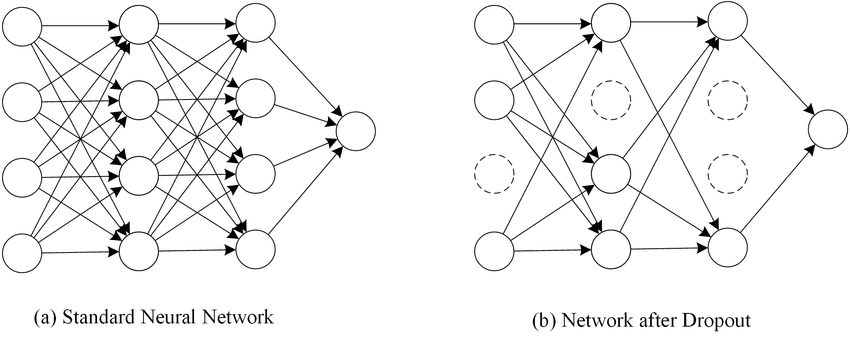
\includegraphics[width=120mm]{lectures/02-b/Dropout.png}
\caption{Neural network dropout}
\label{fig:dropout}
\end{figure}

Dropout has the effect of making the training process noisy, forcing nodes within a layer to probabilistically take on more responsibility for the inputs. 
It helps to spread the evidence to multiple features and prevents the network from giving too much importance to a particular feature. 
It also provides a cheap way of ensembling multiple networks. 
Dropout also helps reduce interdependent learning amongst the neurons and limits the networks ability to memorize very specific conditions during the training. 
As we turn-off some of the hidden units (with some probability), the hidden units are less inclined to learn every redundant detail of instances in training set. 
The subsequent layers will have access to lesser details of the input instance, they increase their efficiency learning to find patterns for unseen data, which gives a boost in generalization.

Dropout may be implemented on any or all hidden layers in the network as well as the visible or input layer. It is not used on the output layer. 
A new hyperparameter is introduced that specifies the probability at which outputs of the layer are dropped out, or inversely, the probability at which outputs of the layer are retained. 
Dropout is not used after training when making a prediction with the fit network. 
The weights of the network will be larger than normal because of dropout. 
Therefore, before finalizing the network, the weights are first scaled by the chosen dropout rate. 
The network can then be used as per normal to make predictions.

{\centering\fbox{\begin{minipage}{30em}
\centering\textbf{Use “dropout” for Regularization}
\begin{enumerate}
    \item A layer that randomly masks out some percentage of the units in the layer and “ignores” them during a pass.
    \item Helps prevent the network from giving too much importance to a particular feature, and incentives to spread the evidence to multiple features
\end{enumerate}
\end{minipage}}\par}

% Authors: tn1050@nyu.edu, vy404@nyu.edu, sk7685@nyu.edu.
% Lecture date: 2.4.19
\section{Schedule To Decrease Learning Rate}
Some tricks are not well understood theoretically and are based on intuition supported by empirical evidence. 
One such trick is decreasing the learning rate during the training. 
When we observe the loss of the neural net plateaus and stops decreasing, it might be helpful to continue training with a lower learning rate. 

\begin{figure}[hbt!]
\centering
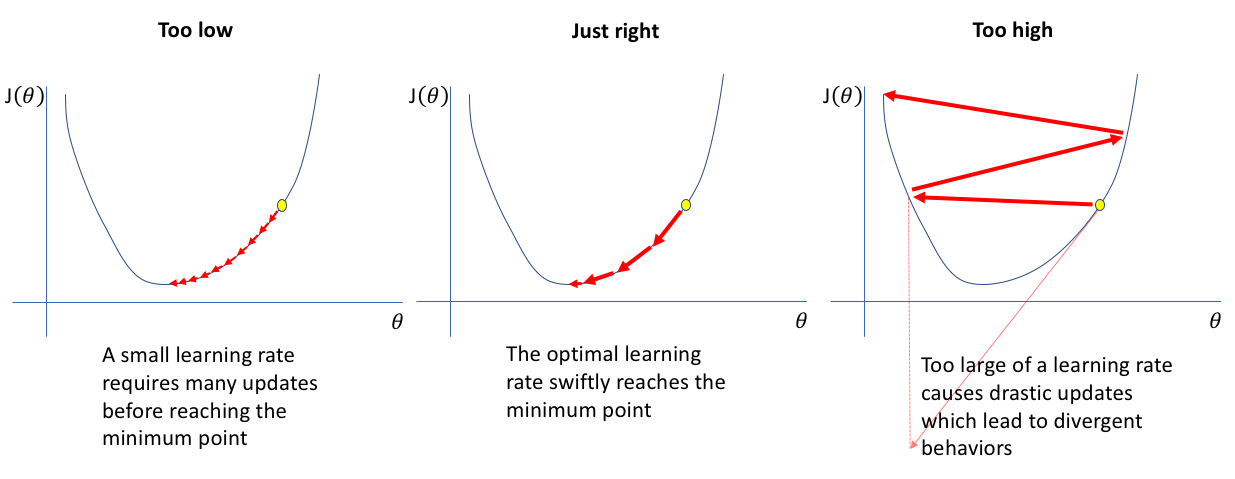
\includegraphics[width=120mm]{lectures/02-b/Learning rate_3.png}
\caption{Gradient descent with small (left), optimal (middle) and large (right) learning rates}
\label{fig:learningrate1}
\end{figure}

To understand why this might be helpful, imagine there are two minima (one deep and narrow and another shallow and wider) and we are optimizing the model parameters with SGD.
Note that the noise in the gradients will be causing the parameters to fluctuate. 
The fluctuations will be smaller in the wider shallower minima than the narrow and deeper one as the weights will be bouncing off sharper in the narrower one, and they might bounce so much that the parameters will go out of the curvature. 
In the wider shallower minima it is very likely that the fluctuations will be smaller even though the minima is higher.

\begin{figure}[hbt!]
\centering
\begin{subfigure}{.5\textwidth}
  \centering
  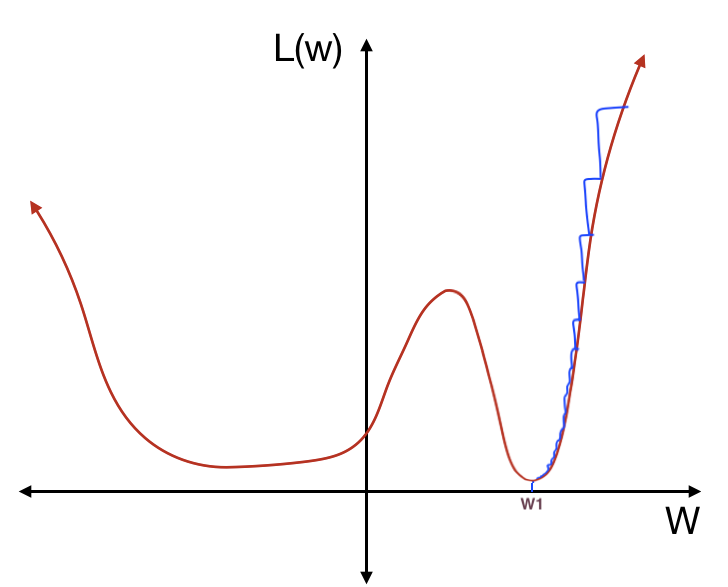
\includegraphics[width=.5\linewidth]{lectures/02-b/Learning rate_1.png}
  \caption{}
  \label{fig:learningrateSub1}
\end{subfigure}%
\begin{subfigure}{.5\textwidth}
  \centering
  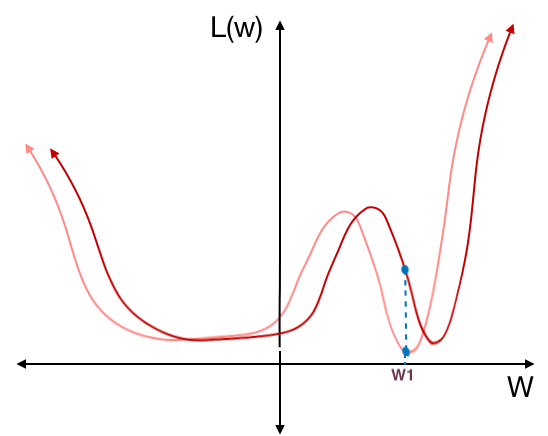
\includegraphics[width=.5\linewidth]{lectures/02-b/Learning rate.png}
  \caption{}
  \label{fig:learningrateSub2}
\end{subfigure}
\caption{(a) Approaching a local minimum with changing step size (b) Slight shift in loss function resulting in a large change in loss}
\label{fig:learningrate2}
\end{figure}

Another thing to consider is that the average loss will be higher for the steeper minima than the shallower minima. 
When we stop the system at one point we might get a higher loss due to bouncing. 
For this reason, some people say that we should not use the last value of the parameters that we obtain through SGD and instead use the average of the past few values by keeping a running average. 
This will help us get closer to the minimum point of a steeper minima. 
This, however, does not guarantee a better test loss, as the loss function that we have in the test set would be different than that of the training set. 
Even if it has the same shape, it might be shifted by a bit. 
Such a shift would affect the loss value more if we are in a steeper minima point. 
One intuition is that we might have a regularization effect when the system wants to choose wider minima as it has a better chance of generalizing properly. 
Another intuition is that regardless of which minima you are in, if you want to get to it quickly, a large learning rate might help the system approach the minima but may not let it go inside the minima because of the large fluctuation and we need to decrease the learning rate so it can settle in the minima.

{\centering\fbox{\begin{minipage}{30em}
\centering\textbf{Schedule To Decrease Learning Rate}
\begin{enumerate}
    \item When the loss of the neural net plateaus, it might be helpful to continue training with a lower learning rate.
    \item Slight shift in loss function of test set results in a large change in loss.
\end{enumerate}
\end{minipage}}\par}
\vspace{5pt}

One reason why neural nets disappeared in the mid-90s was because of few people who had developed tricks to make neural nets run on their system however any people who tried new neural nets would not know them and would need to figure them out themselves. 
That led to people just giving up. 